%% supplement.tex — Online Supplement
%% Lancet Regional Health – Americas
%% ===================================================================
\documentclass[12pt]{article}

\usepackage[utf8]{inputenc}
\usepackage[T1]{fontenc}
\usepackage{amsmath,amssymb}
\usepackage{graphicx}
\usepackage{booktabs}
\usepackage{multirow}
\usepackage{xcolor}
\usepackage{hyperref}
\usepackage[margin=2.5cm]{geometry}
\usepackage{caption}

%% Prefix tables and figures with "e"
\renewcommand{\thetable}{e\arabic{table}}
\renewcommand{\thefigure}{e\arabic{figure}}

\begin{document}

\begin{center}
{\Large\bfseries Online Supplement}\\[0.5em]
{\large Non-Linear and Delayed Effects of Cold Extremes on Respiratory
Hospital Admissions in a Subtropical Metropolis: A Quasi-Poisson
Time-Series Analysis in Curitiba, Brazil}\\[0.5em]
Felipe Baglioli, Lucas Rover\\
Federal University of Paran\'{a} (UFPR), Curitiba, PR, Brazil
\end{center}

\bigskip

%% ═══════════════════════════════════════════════════════════════════
%% SUPPLEMENTARY METHODS
%% ═══════════════════════════════════════════════════════════════════
\section*{Supplementary Methods}

\subsection*{Machine learning forecasting details}

\paragraph{Extreme Learning Machine (ELM)}
A single-hidden-layer feedforward network with random input weights
and regularised pseudoinverse output weights. Hyperparameter: number
of hidden neurons (scanned over 1--200).

\paragraph{Multilayer perceptron (MLP)}
A PyTorch-based feedforward network with one hidden layer (tanh
activation), trained with Adam optimiser (learning rate 0${\cdot}$01),
mini-batch size 20, early stopping (patience 10), and learning-rate
scheduling.

\paragraph{XGBoost}
A gradient-boosted tree ensemble (max depth 5, learning rate
0${\cdot}$1, \texttt{reg:squarederror} objective). The number of
estimators was tuned via validation-set MSE.

\paragraph{Training protocol}
Data were split temporally: 70\% training, 15\% validation, 15\%
test. Features were standardised (zero mean, unit variance). Model
selection used MAPE on the validation set; final evaluation used the
test set after retraining on training+validation data. SHAP (SHapley
Additive exPlanations) values were computed for the XGBoost model to
quantify feature importance.

\paragraph{Climate projections}
Future temperature scenarios were derived from the CMIP6 SSP5-8${\cdot}$5
pathway (EC-Earth3-Veg-LR model) for Curitiba's grid cell, with daily
$T_\mathrm{max}$, $T_\mathrm{med}$, and specific humidity extracted
for 2030, 2050, and 2099. Future PM$_{2{\cdot}5}$ was projected using
the most recent year's Transformer-imputed series as baseline.

\paragraph{Monte Carlo extreme-event simulations}
Heat waves were simulated by injecting random temperature perturbations
(+2--5\,°C for 3--7~days) during autumn; cold waves by analogous
decrements during spring/autumn. Wildfire PM$_{2{\cdot}5}$ spikes were
simulated by adding 70--100~µg/m$^3$ pulses (7--14~days) during
summer/spring.

\subsection*{Clustering and PCA}

K-means clustering was applied to six standardised variables
($T_\mathrm{max}$, $T_\mathrm{med}$, $T_\mathrm{min}$,
PM$_{2{\cdot}5}$, relative humidity, atmospheric pressure) on
$N$=558 complete-case days. Optimal $K$=3 was selected by silhouette
score (0${\cdot}$357). Three clusters emerged: Clean Cold ($n$=248),
Polluted Heat ($n$=12), and Clean Heat ($n$=298). Kruskal--Wallis
test for between-cluster differences in daily hospitalisations
yielded $p$=0${\cdot}$039 (eTables~2--3). PCA on PM$_{2{\cdot}5}$,
$T_\mathrm{min}$, and hospitalisations identified PC1 (44${\cdot}$5\%
variance) associating cold, polluted days with higher admissions
(eTable~4). Extended lag correlations (eTable~5) revealed peak
$T_\mathrm{min}$--hospitalisation correlation at lag~9
($r$=$-$0${\cdot}$320, $p<$0${\cdot}$001).

\subsection*{Exploratory PM$_{2{\cdot}5}$ DLNM}

An exploratory DLNM for EPA-corrected PM$_{2{\cdot}5}$ ($N$=697,
lag 0--14~days, exposure df=4, lag df=4) showed no significant
cumulative associations at any percentile (eFigure~6): P90
(10${\cdot}$2~µg/m$^3$) RR=0${\cdot}$91 [0${\cdot}$78--1${\cdot}$07].
The low ambient concentrations (median 4${\cdot}$1~µg/m$^3$, well
below the WHO 24-hour guideline) and 36${\cdot}$4\% missing data
likely limited statistical power. A joint model ($N$=683) yielded
RERI=0${\cdot}$013 [$-$0${\cdot}$006, 0${\cdot}$033] on the additive
scale, indicating no evidence of supra-additive interaction between
temperature and PM$_{2{\cdot}5}$ (eTable~6).

\subsection*{Missing data sensitivity}

Sensitivity analyses with mean imputation and $k$-nearest-neighbour
imputation ($k$=5) produced qualitatively similar clustering solutions
to the primary complete-case analysis (silhouette scores within
0${\cdot}$02 of the main analysis). PCA loadings and explained
variance were robust to imputation method.

%% ═══════════════════════════════════════════════════════════════════
%% SUPPLEMENTARY TABLES
%% ═══════════════════════════════════════════════════════════════════
\clearpage
\section*{Supplementary Tables}

\begin{table}[ht]
\centering
\caption{Summary of extreme temperature events, Curitiba, 2022--2024.
Heatwaves: $\geq$3 consecutive days with $T_\mathrm{max}$~$>$~TX90p;
cold spells: $\geq$3 consecutive days with $T_\mathrm{min}$~$<$~TN10p.}
\label{etab:extreme_events}
\begin{tabular}{lrrrr}
\toprule
Event type & Count & Total days & Mean duration & Range (days) \\
\midrule
Heatwaves    & 25 & 215 & 4${\cdot}$5 & 3--17 \\
Cold spells  &  4 &  39 & 4${\cdot}$0 & 3--7 \\
\bottomrule
\end{tabular}
\end{table}

\begin{table}[ht]
\centering
\caption{Cluster profiles at $K$=3 (optimal by silhouette, $N$=558
complete-case days). Temperature in °C (INMET); PM$_{2{\cdot}5}$
EPA-corrected.}
\label{etab:clusters_k3}
\begin{tabular}{lrrrrrrr}
\toprule
Cluster & $n$ & $T_\mathrm{max}$ & $T_\mathrm{med}$ &
  $T_\mathrm{min}$ & PM$_{2{\cdot}5}$ & RH (\%) & Pressure \\
  & & (°C) & (°C) & (°C) & (µg/m$^3$) & & (hPa) \\
\midrule
0 -- Clean Cold     & 248 & 21${\cdot}$3 & 16${\cdot}$2 & 12${\cdot}$7 &  4${\cdot}$8 & 83${\cdot}$4 & 914${\cdot}$6 \\
1 -- Polluted Heat  &  12 & 30${\cdot}$0 & 21${\cdot}$5 & 13${\cdot}$4 & 51${\cdot}$5 & 57${\cdot}$4 & 915${\cdot}$4 \\
2 -- Clean Heat     & 298 & 28${\cdot}$3 & 21${\cdot}$9 & 17${\cdot}$9 &  4${\cdot}$9 & 79${\cdot}$2 & 911${\cdot}$2 \\
\bottomrule
\end{tabular}
\end{table}

\begin{table}[ht]
\centering
\caption{Cluster profiles at $K$=4 (manuscript validation).
Kruskal--Wallis $H$=16${\cdot}$69, $p<$0${\cdot}$001 for
between-cluster differences in daily hospitalisations.}
\label{etab:clusters_k4}
\begin{tabular}{lrrrrrr}
\toprule
Cluster & $n$ & $T_\mathrm{max}$ & $T_\mathrm{med}$ &
  PM$_{2{\cdot}5}$ & RH (\%) & Hosp/day \\
  & & (°C) & (°C) & (µg/m$^3$) & & (mean $\pm$ SD) \\
\midrule
Clean Cold     & 197 & 23${\cdot}$3 & 18${\cdot}$4 &  3${\cdot}$2 & 86${\cdot}$4 & 31${\cdot}$3 $\pm$ 11${\cdot}$2 \\
Clean Heat     & 221 & 29${\cdot}$5 & 22${\cdot}$6 &  5${\cdot}$4 & 76${\cdot}$7 & 29${\cdot}$4 $\pm$ 10${\cdot}$5 \\
Polluted Heat  &  12 & 30${\cdot}$0 & 21${\cdot}$5 & 51${\cdot}$5 & 57${\cdot}$4 & 38${\cdot}$6 $\pm$ 9${\cdot}$7 \\
Moderate Trans. & 128 & 20${\cdot}$5 & 14${\cdot}$9 &  6${\cdot}$5 & 80${\cdot}$6 & 33${\cdot}$8 $\pm$ 11${\cdot}$7 \\
\bottomrule
\end{tabular}
\end{table}

\begin{table}[ht]
\centering
\caption{PCA loadings and explained variance ($N$=683 complete-case
days). Variables standardised prior to decomposition.}
\label{etab:pca}
\begin{tabular}{lcccc}
\toprule
Component & PM$_{2{\cdot}5}$ & $T_\mathrm{min}$ & Hospitalisations & Explained Var. \\
\midrule
PC1 & $+$0${\cdot}$564  & $-$0${\cdot}$580 & $+$0${\cdot}$588 & 44${\cdot}$5\% \\
PC2 & $+$0${\cdot}$810  & $+$0${\cdot}$525 & $-$0${\cdot}$259 & 28${\cdot}$2\% \\
\bottomrule
\end{tabular}
\end{table}

\begin{table}[ht]
\centering
\caption{Extended lag correlations (Pearson $r$) between exposures and
daily hospitalisations, selected lags. Bold: significant at $p<$0${\cdot}$05.}
\label{etab:extended_lags}
\begin{tabular}{lrrrrrr}
\toprule
 & \multicolumn{3}{c}{PM$_{2{\cdot}5}$ EPA} & \multicolumn{3}{c}{$T_\mathrm{min}$} \\
\cmidrule(lr){2-4} \cmidrule(lr){5-7}
Lag (days) & $r$ & $p$ & $N$ & $r$ & $p$ & $N$ \\
\midrule
 0 & \textbf{$+$0${\cdot}$159} & $<$0${\cdot}$001 & 697 & \textbf{$-$0${\cdot}$231} & $<$0${\cdot}$001 & 1066 \\
 3 & \textbf{$+$0${\cdot}$141} & $<$0${\cdot}$001 & 694 & \textbf{$-$0${\cdot}$306} & $<$0${\cdot}$001 & 1063 \\
 6 & \textbf{$+$0${\cdot}$165} & $<$0${\cdot}$001 & 691 & \textbf{$-$0${\cdot}$282} & $<$0${\cdot}$001 & 1060 \\
 9 &  $+$0${\cdot}$069 & 0${\cdot}$071 & 688 & \textbf{$-$0${\cdot}$320} & $<$0${\cdot}$001 & 1057 \\
13 & \textbf{$+$0${\cdot}$172} & $<$0${\cdot}$001 & 684 & \textbf{$-$0${\cdot}$232} & $<$0${\cdot}$001 & 1053 \\
21 &  $+$0${\cdot}$080 & 0${\cdot}$037 & 676 & \textbf{$-$0${\cdot}$225} & $<$0${\cdot}$001 & 1045 \\
28 &  $+$0${\cdot}$085 & 0${\cdot}$029 & 669 & \textbf{$-$0${\cdot}$183} & $<$0${\cdot}$001 & 1038 \\
\bottomrule
\end{tabular}
\end{table}

\begin{table}[ht]
\centering
\caption{Interaction analysis on the additive scale (RERI). Joint
quasi-Poisson DLNM, $N$=683.}
\label{etab:reri}
\begin{tabular}{lrrr}
\toprule
Metric & Estimate & 95\% CI lower & 95\% CI upper \\
\midrule
RERI & 0${\cdot}$013 & $-$0${\cdot}$006 & 0${\cdot}$033 \\
AP   & 0${\cdot}$019 &  ---     &  ---  \\
S    & 0${\cdot}$955 &  ---     &  ---  \\
\bottomrule
\end{tabular}
\end{table}

\begin{table}[ht]
\centering
\caption{Model diagnostics for the quasi-Poisson DLNM.}
\label{etab:diagnostics}
\begin{tabular}{lrrrrr}
\toprule
Model & $\hat{\phi}$ & DW & Ljung--Box $p$ & ACF lag\,1 & ACF lag\,7 \\
\midrule
Temperature & 1${\cdot}$322 & 2${\cdot}$004 & 0${\cdot}$137 & $-$0${\cdot}$006 & 0${\cdot}$077 \\
PM$_{2{\cdot}5}$  & 1${\cdot}$329 & 2${\cdot}$115 & 0${\cdot}$096 & $-$0${\cdot}$059 & 0${\cdot}$025 \\
\bottomrule
\end{tabular}
\end{table}

\begin{table}[ht]
\centering
\caption{Machine learning model performance for daily respiratory
hospitalisation forecasting, Curitiba, 2022--2024. Best result per
metric in bold.}
\label{etab:ml_results}
\begin{tabular}{llrrrr}
\toprule
Lag & Model & RMSE & MAE & MAPE (\%) & $N_\mathrm{param}$ \\
\midrule
0 & ELM     & 11${\cdot}$07 &  8${\cdot}$95 & 30${\cdot}$9 & 182 \\
0 & MLP     &  9${\cdot}$31 &  7${\cdot}$53 & 25${\cdot}$1 &   6 \\
0 & \textbf{XGBoost} & \textbf{8${\cdot}$37} & \textbf{6${\cdot}$30} & \textbf{19${\cdot}$4} &  29 \\
\midrule
1 & ELM     & 10${\cdot}$43 &  8${\cdot}$30 & 28${\cdot}$1 & 182 \\
1 & MLP     &  8${\cdot}$80 &  7${\cdot}$01 & 23${\cdot}$2 &   4 \\
1 & \textbf{XGBoost} & \textbf{8${\cdot}$10} & \textbf{6${\cdot}$10} & \textbf{18${\cdot}$0} &  18 \\
\midrule
5 & ELM     & 10${\cdot}$74 &  8${\cdot}$68 & 28${\cdot}$8 & 186 \\
5 & \textbf{MLP} & \textbf{8${\cdot}$14} & \textbf{6${\cdot}$09} & \textbf{19${\cdot}$1} &   3 \\
5 & XGBoost &  8${\cdot}$42 &  6${\cdot}$47 & 20${\cdot}$3 &  18 \\
\midrule
7 & ELM     & 10${\cdot}$28 &  7${\cdot}$99 & 26${\cdot}$3 &  94 \\
7 & MLP     &  9${\cdot}$67 &  7${\cdot}$60 & 24${\cdot}$6 &  12 \\
7 & \textbf{XGBoost} & \textbf{8${\cdot}$66} & \textbf{6${\cdot}$57} & \textbf{20${\cdot}$8} &  19 \\
\bottomrule
\end{tabular}
\end{table}

%% ═══════════════════════════════════════════════════════════════════
%% SUPPLEMENTARY FIGURES
%% ═══════════════════════════════════════════════════════════════════
\clearpage
\section*{Supplementary Figures}

\begin{figure}[ht]
\centering
\includegraphics[width=\textwidth]{../analysis/clustering/figures/fig_elbow_silhouette.pdf}
\caption{Cluster selection metrics for $K$=2--10: (a) elbow plot of
within-cluster inertia, (b) silhouette score (optimal at $K$=3),
(c) Calinski--Harabasz index, and (d) Davies--Bouldin index.}
\label{efig:k_selection}
\end{figure}

\begin{figure}[ht]
\centering
\includegraphics[width=0.85\textwidth]{../analysis/clustering/figures/fig_cluster_pca.pdf}
\caption{PCA biplot of cluster assignments ($K$=3). Loading vectors
show the contribution of each variable to PC1 (35${\cdot}$9\%) and
PC2 (22${\cdot}$4\%).}
\label{efig:cluster_pca}
\end{figure}

\begin{figure}[ht]
\centering
\includegraphics[width=\textwidth]{../analysis/clustering/figures/fig_method_comparison.pdf}
\caption{Comparison of clustering methods ($K$=3): K-means
(silhouette=0${\cdot}$357), Ward hierarchical (0${\cdot}$321), and
DBSCAN (single cluster).}
\label{efig:method_cmp}
\end{figure}

\begin{figure}[ht]
\centering
\includegraphics[width=\textwidth]{../analysis/clustering/figures/fig_lag_correlation.pdf}
\caption{Lag correlations (lags 0--14~days) between cluster membership
and daily hospitalisations: (a) Pearson $r$ and (b) Spearman $\rho$.}
\label{efig:lag_corr}
\end{figure}

\begin{figure}[ht]
\centering
\includegraphics[width=\textwidth]{../analysis/dlnm/figures/fig_dlnm_temp_3d.pdf}
\caption{(a) Contour plot and (b) 3D surface of RR across temperature
and lag dimensions.}
\label{efig:dlnm_temp_3d}
\end{figure}

\begin{figure}[ht]
\centering
\includegraphics[width=0.85\textwidth]{../analysis/dlnm/figures/fig_dlnm_pm25_overall.pdf}
\caption{Cumulative exposure--response curve for EPA-corrected
PM$_{2{\cdot}5}$ and respiratory hospitalisations (DLNM, lag
0--14~days).}
\label{efig:dlnm_pm25_overall}
\end{figure}

\begin{figure}[ht]
\centering
\includegraphics[width=0.85\textwidth]{../analysis/dlnm/figures/fig_stationarity.pdf}
\caption{Stationarity assessment: (a) observed hospitalisations with
STL trend, (b) seasonal component, (c) STL residuals (ADF
$p$=0${\cdot}$0003), and (d) lag correlations for raw vs.\ detrended
series.}
\label{efig:stationarity}
\end{figure}

\begin{figure}[ht]
\centering
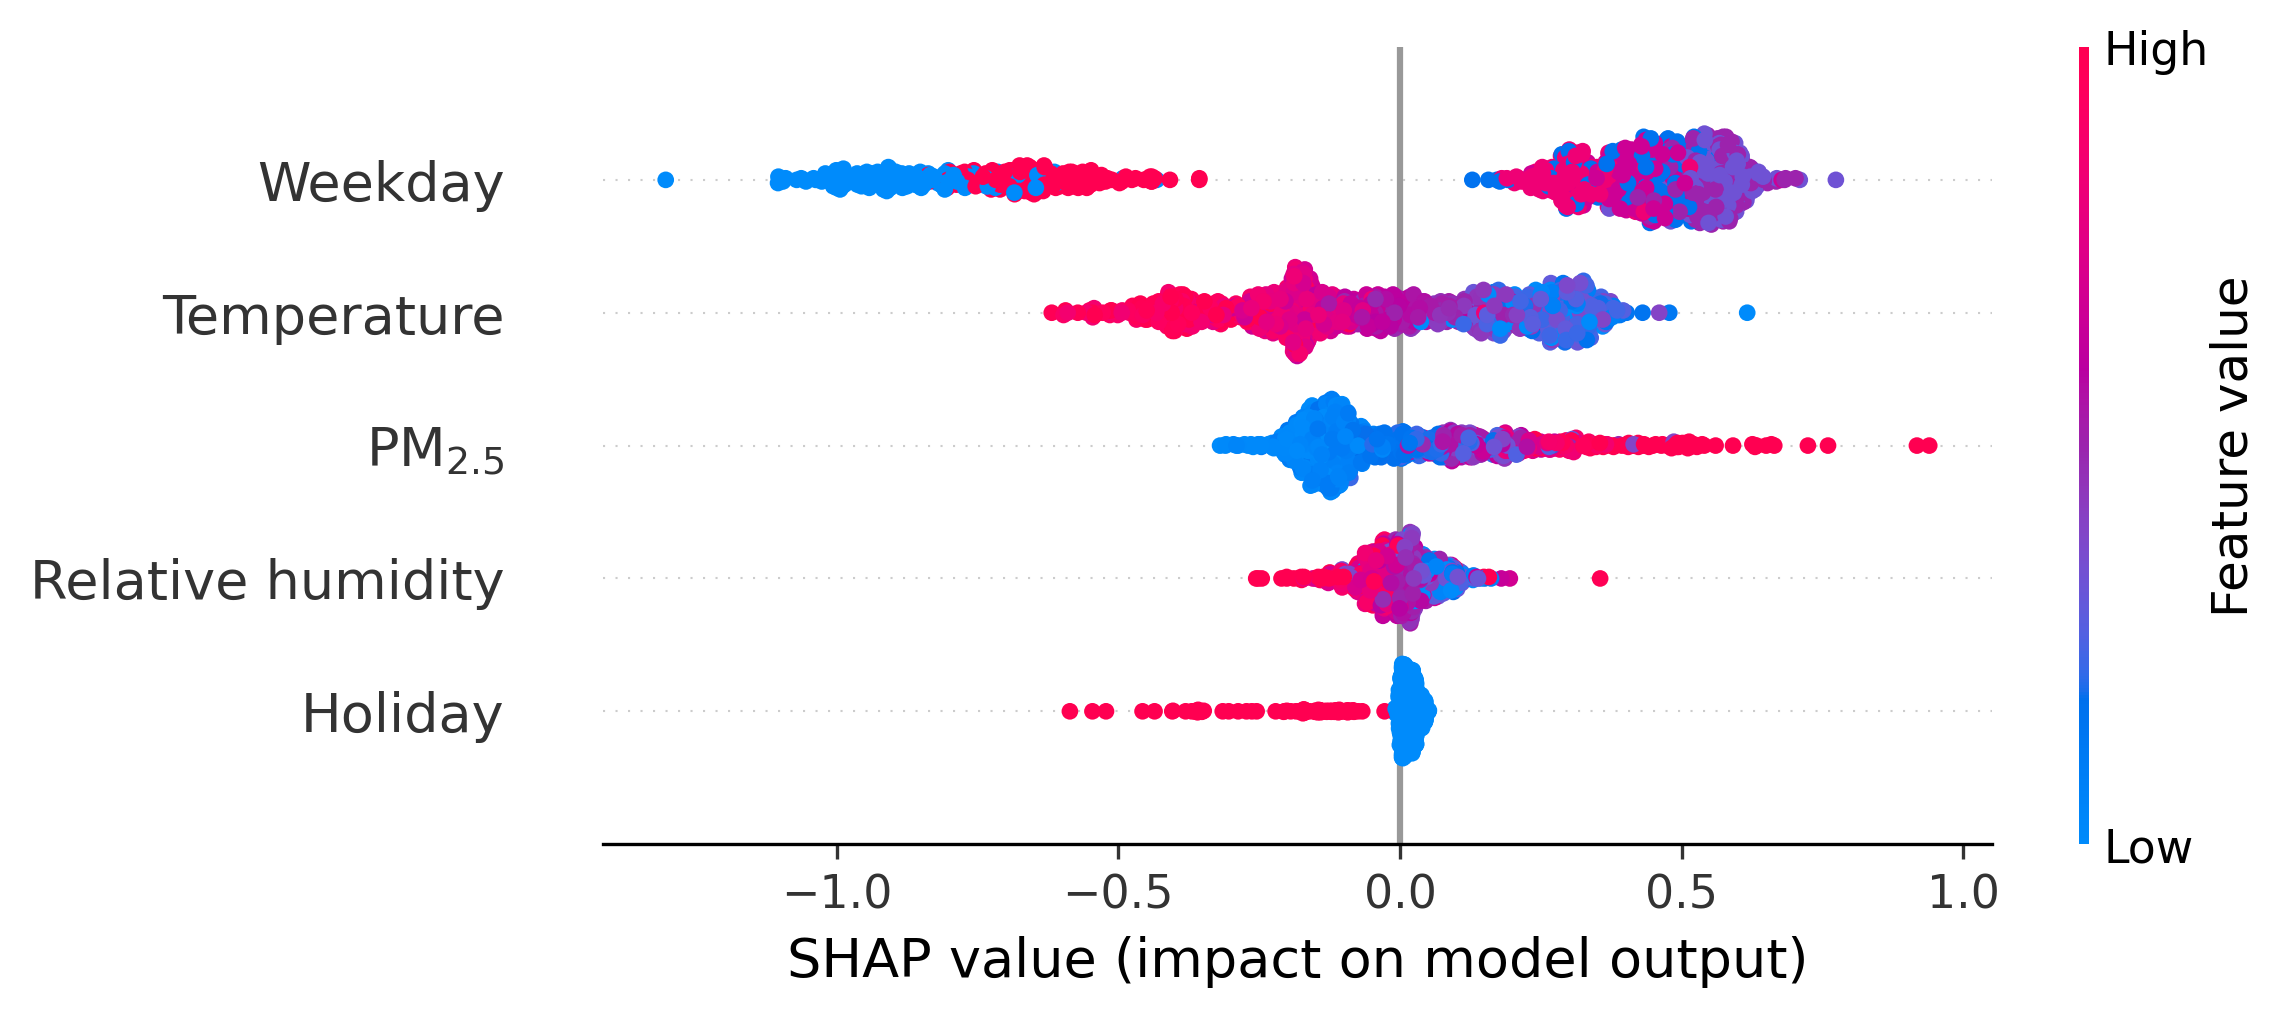
\includegraphics[width=0.85\textwidth]{../analysis/forecasting_pm25/shap_summary_curitiba_lag0.png}
\caption{SHAP summary plot (beeswarm) for the XGBoost model at lag~0.
Each dot represents one day; colour indicates feature value (blue =
low, red = high). Features ranked by mean absolute SHAP value.}
\label{efig:shap}
\end{figure}

\end{document}
